\documentclass[11pt,article,oneside,british,extralanguage=dutch]{kulemt}
\usepackage[kuldate]{kulemtx}
\usepackage{rotating}
\usepackage{layouts}

%% Fonts 
%  - Select the main text and math fonts
%    Remember their names, so we can use them in the text
\usepackage{libertinus}
\newcommand*\rmfontname{Libertinus Serif}
\newcommand*\sffontname{Libertinus Sans}
\IfPackageLoadedTF{fontspec}%
  {%
    \usepackage{unicode-math}%
    \setmathfont{Libertinus Math}%
    \setmonofont{Latin Modern Mono}%
    \newcommand*\ttfontname{Latin Modern Mono}%
  }%
  {%
    \usepackage{libertinust1math}%
    \renewcommand{\ttdefault}{lmtt}%
    \newcommand*\ttfontname{Latin Modern Typewriter}%
  }
%  - Use microtype to enhance the typography
\usepackage{microtype}
%  - Generate an error for missing glyphs
\tracinglostchars=3

%% Finally hyperref is loaded for proper PDF links
%  Colors: external links in blue, internal ones in dark blue
\usepackage[pdfusetitle]{hyperref}
\hypersetup{colorlinks,%
  filecolor={[rgb]{0,0,1}},urlcolor={[rgb]{0,0,1}},%
  citecolor={[rgb]{0,0,.75}},linkcolor={[rgb]{0,0,.75}}}

%% Styling pages, sections and lists
\pagestyle{plain}
\renewcommand\chaptitlefont{\Large\sffamily}
\setsecheadstyle{\large\sffamily\raggedright}
\setsubsecheadstyle{\large\sffamily\itshape\raggedright}
\setparaheadstyle{\normalsize\scshape}
\setbeforeparaskip{\medskipamount}
\firmlists

%% Footnote
%  Set the marker flushleft and the text as a block paragraph
\setlength\footmarkwidth{1.5ex}
\setlength\footmarksep{0pt}
\footmarkstyle{\textsuperscript{#1}\hfill}

%% Define some typesetting commands
%  NOTE: Please do not use logos (\LaTeX ...) in the text, but simply LaTeX ...
\newcommand*\cls[1]{\textsf{#1}}
\newcommand\Dutch[1]{`{\selectlanguage{dutch}#1}'}

\begin{document}
\title{\itshape Guidelines for writing a master's thesis \\
  at the KU~Leuven Faculty of Engineering Science}
\author{Luc Van Eycken}
\maketitle
\bigskip

\noindent The evaluation of the master's thesis depends largely on the quality
of the text. Because the master's thesis equals 25 to 50\,\% of the marks of
the last year, it is important that the presented work is clearly described.
But please refrain from repeating the course material. And of course,
plagiarism will not be tolerated!

\medskip
\makeatletter \renewcommand\@tocmaketitle{} \makeatother
\tableofcontents*
\medskip

\chapter{Contents of the thesis text}
The master's thesis text should be complete, meaning that all of your thesis
work is covered. However it is not a diary but a synthesis of your work.
Therefore you should not make the document needlessly long: you are judged
by the contents, not by the number of pages.

The master's thesis text is not meant to be read only by your jury; it is a
public text. This means that the text must be written in such a way that
any engineer with a degree similar to yours must be able to understand it.
If some of your work cannot be disseminated to the broad public, e.g.\
because of pending patents, you can leave this information out of the text.
But all your results must be communicated to your jury, even the parts
which were removed from your text. So if you leave out important results
from your text, consult your thesis supervisor (\Dutch{promotor}) and
programme director for the exact guidelines.

The language used to write the text in is normally the same as the master's
programme language (namely the official language of the master's programme).
Your master's programme director can allow you to use another text language as
a departure from this rule. This is typically the case for students who prepare
their thesis abroad, such as Erasmus students. But as indicated below, some
items (e.g., the title page) are always typeset in the master's programme
language, even if it differs from the text language.

The following sections describe the elements of the thesis text and the
order in which they must appear in the printed thesis. Unless mentioned
otherwise, all these sections are mandatory. Additionally the master's programme
guidelines must be checked for extra requirements.

\section{Front pages}
The front pages consist of the title page and the copyright page. These
pages have a fixed layout. You can generate them yourself using LaTeX with the
document class \cls{kulemt} or with the Word templates. Both are available from
the website~\cite{templates}.

\paragraph{Cover page (\Dutch{kaft})} The cover page will be printed on the
front of the hard cover of your booklet. Therefore there is no need to include
it in an electronic version. It is a copy of the title page.

\paragraph{Title page} The title page (\fref{fig:titlepage}) is the first page
of the actual document.
\begin{sidewaysfigure}[p]
  \centering \fboxsep=0pt
  \fbox{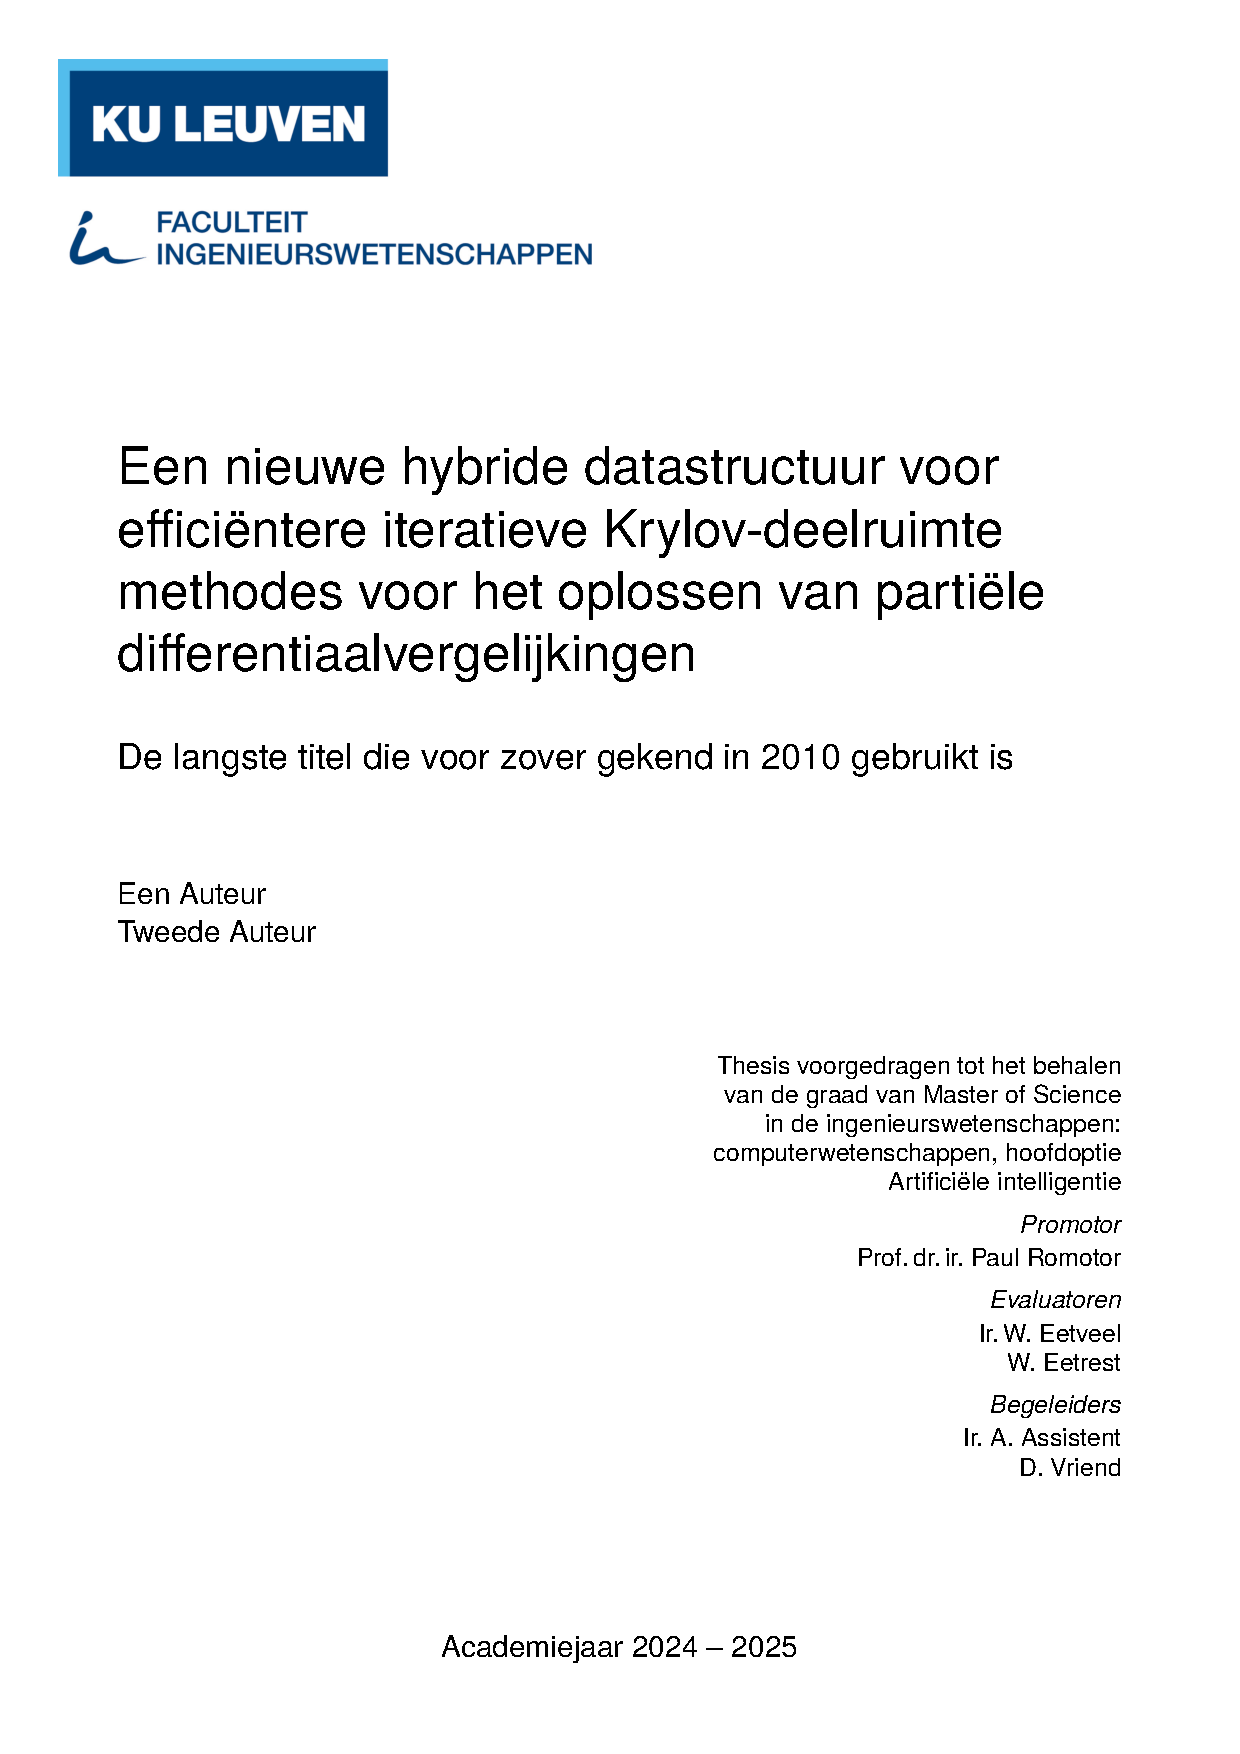
\includegraphics[width=.45\textwidth]{titlepage-nl}}
  \qquad
  \fbox{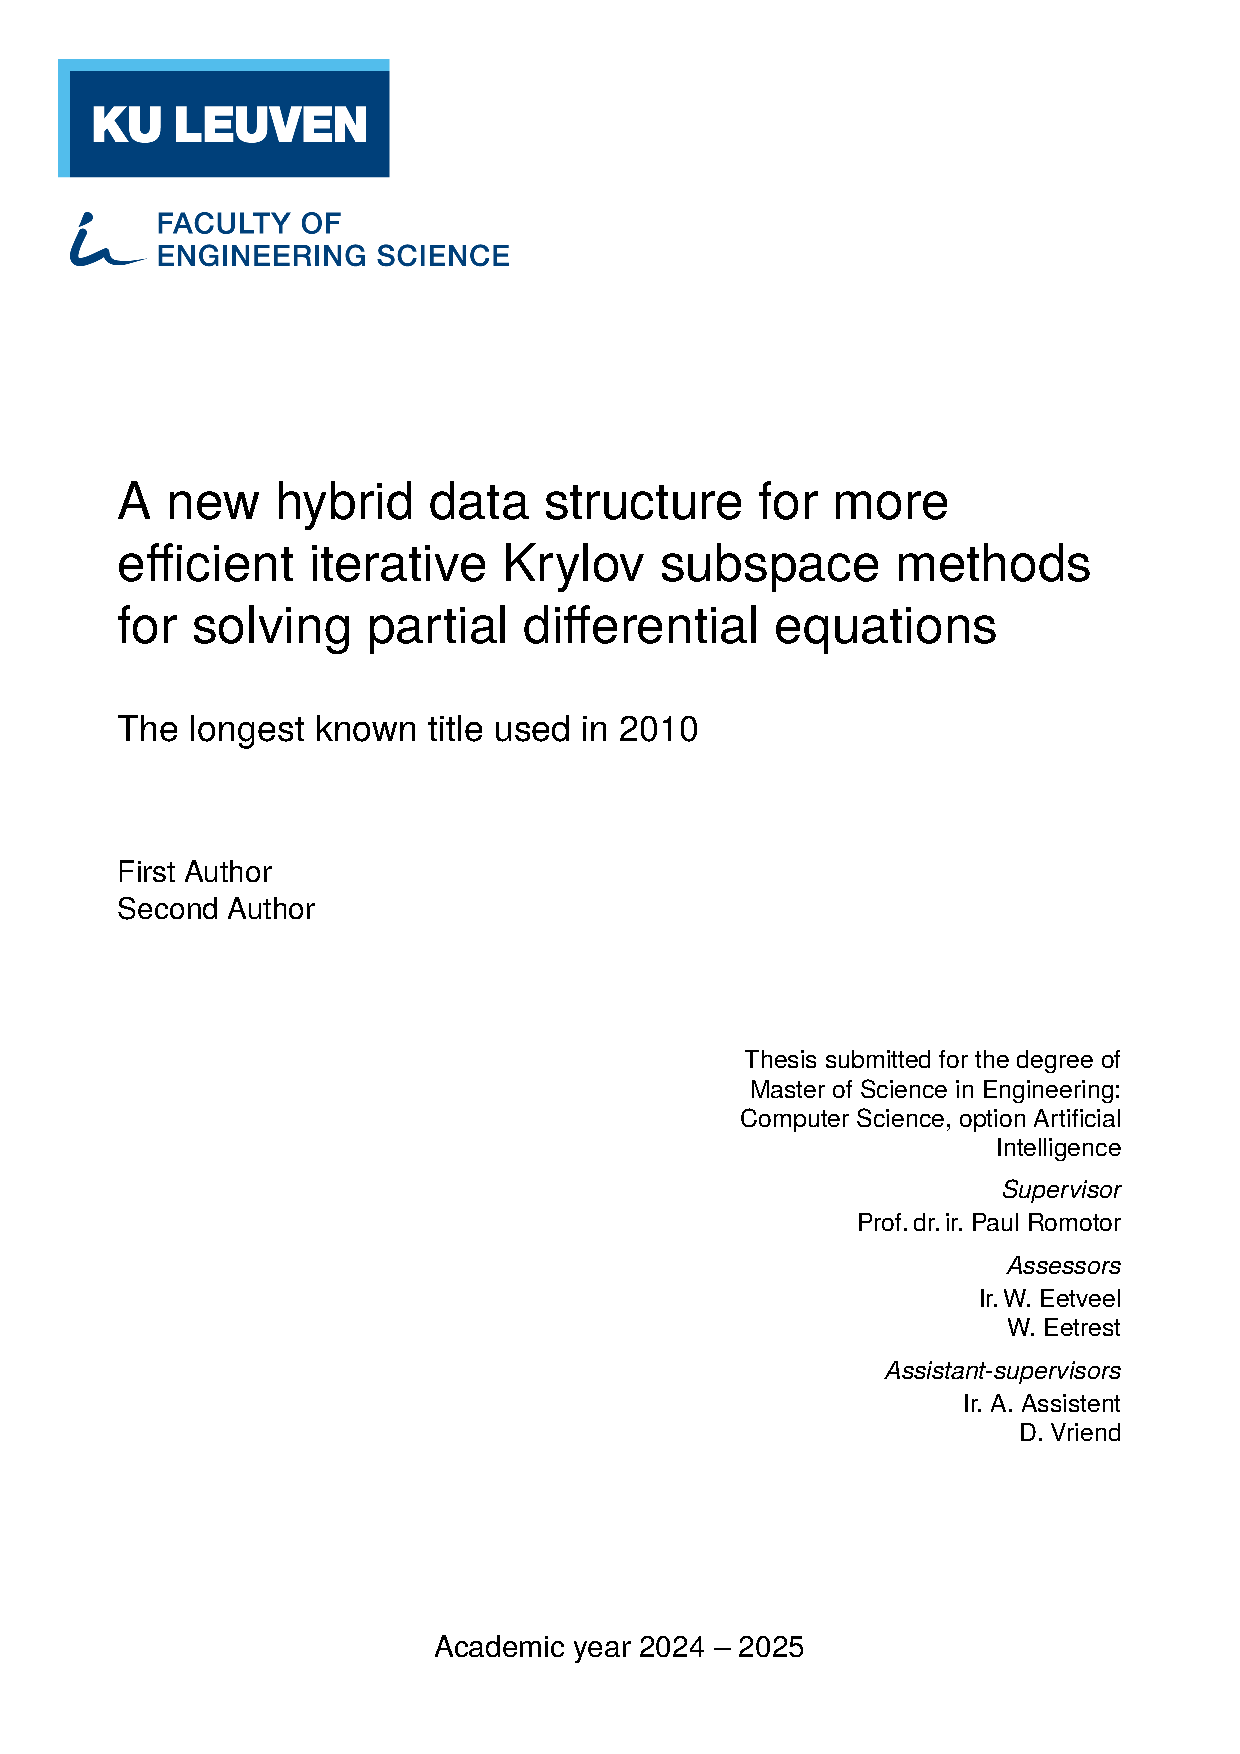
\includegraphics[width=.45\textwidth]{titlepage-en}}
  \caption{The official title page layout for a Dutch master (left) and an
    English master (right). The cover page has exactly the same look.}
  \label{fig:titlepage}
\end{sidewaysfigure}
It contains the necessary logo, an identification of the master's degree, the
academic year, the title (and if wanted a subtitle), and the names of the
students, of the thesis supervisor(s), and of the jury members. The title page
is always typeset in the master's programme language, except for the title and
the subtitle, which are typeset in the text language.

The branding of the Faculty of Engineering Science requires a uniform look of
the title page and the cover page. So not only the layout is fixed, but also
the fonts and font sizes used on those pages. Only Helvetica or Arial (or a
look-alike, such as TeX Gyre Heros) can be used. The title is set in 25\,pt and
the subtitle in 17\,pt. The author(s) and the academic year are set in 14\,pt.
The rest of the title page is set in 11\,pt.

\paragraph{Copyright page}
The copyright page (\fref{fig:copyright}) contains the necessary copyright
statements and contact information. It is printed on the verso side of the
title page. If the text language differs from the master's programme language,
you may provide copyright statements in both languages.
\begin{sidewaysfigure}[p]
  \centering \fboxsep=0pt
  \fbox{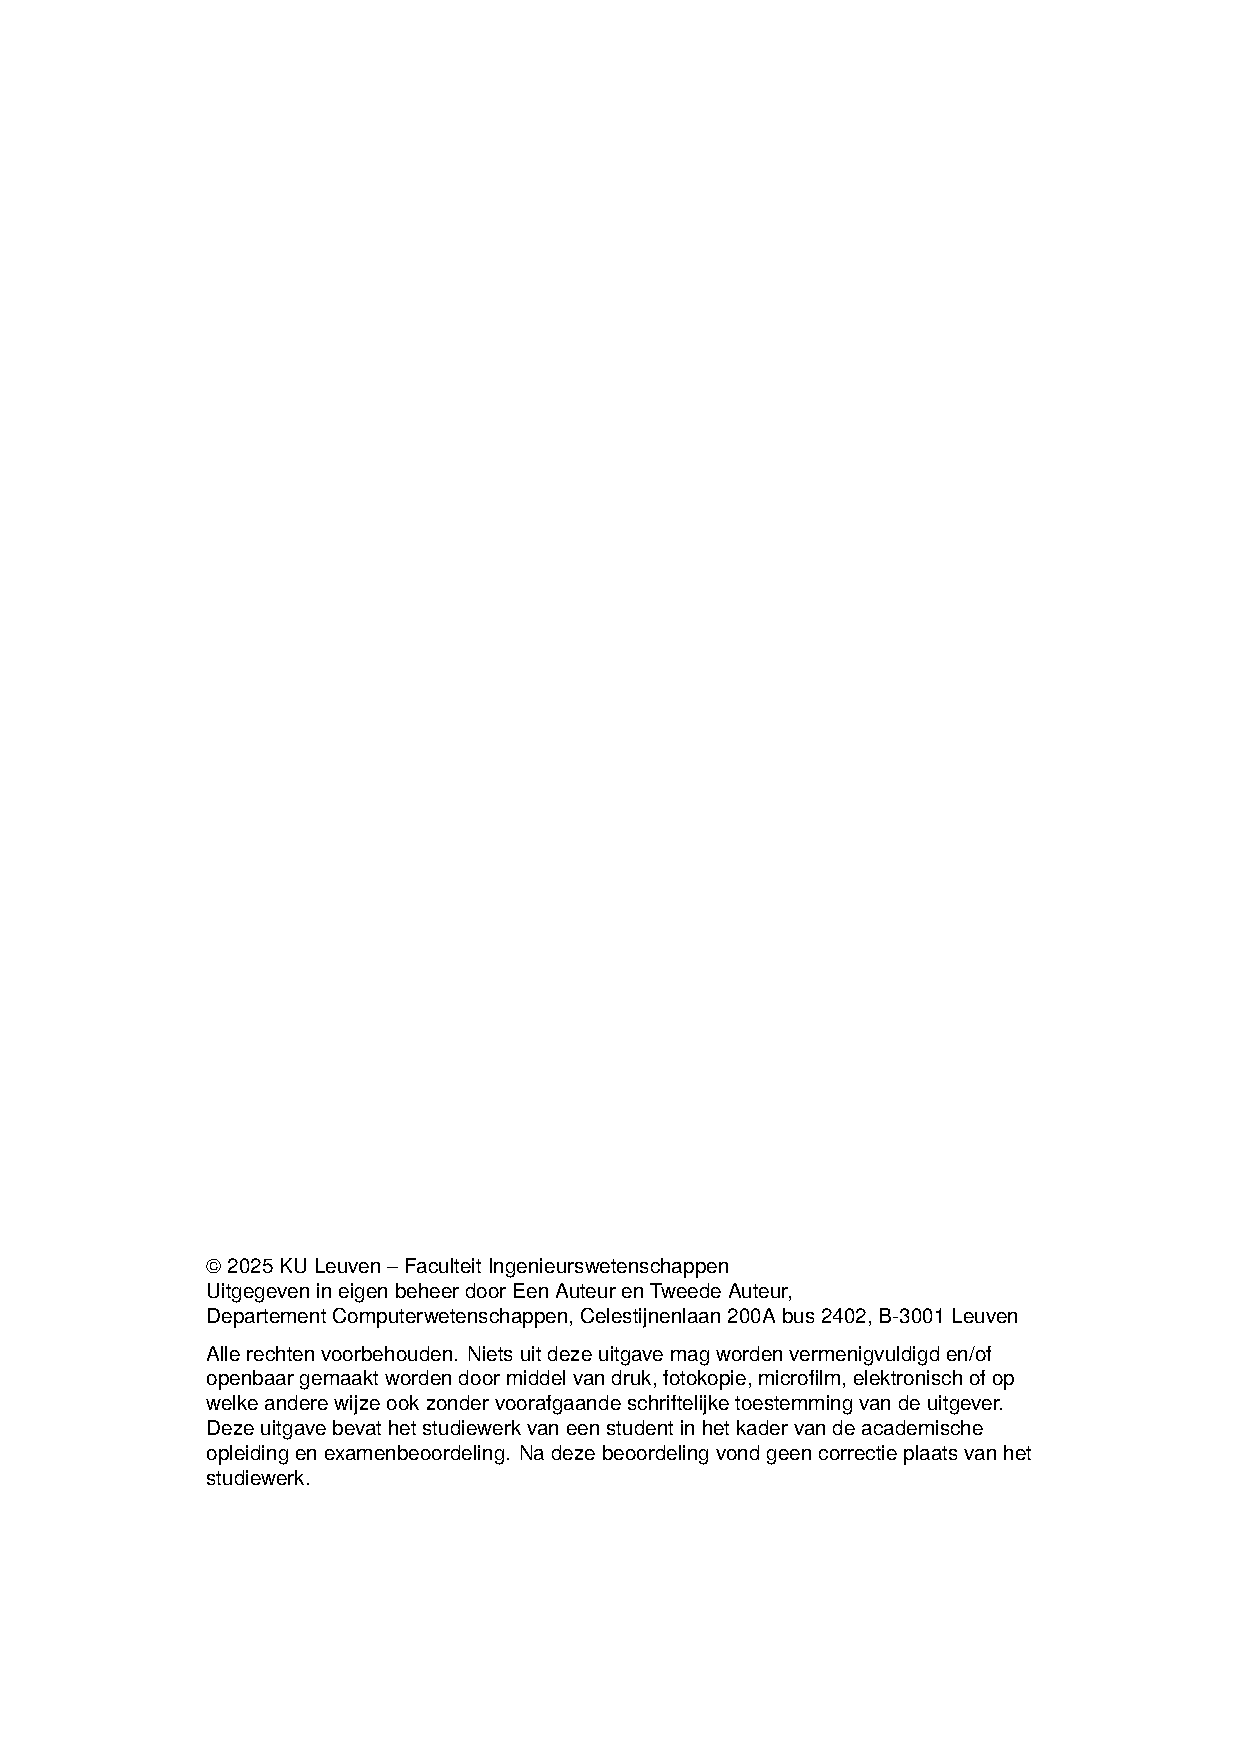
\includegraphics[width=.45\textwidth]{copyright-nl}}
  \qquad
  \fbox{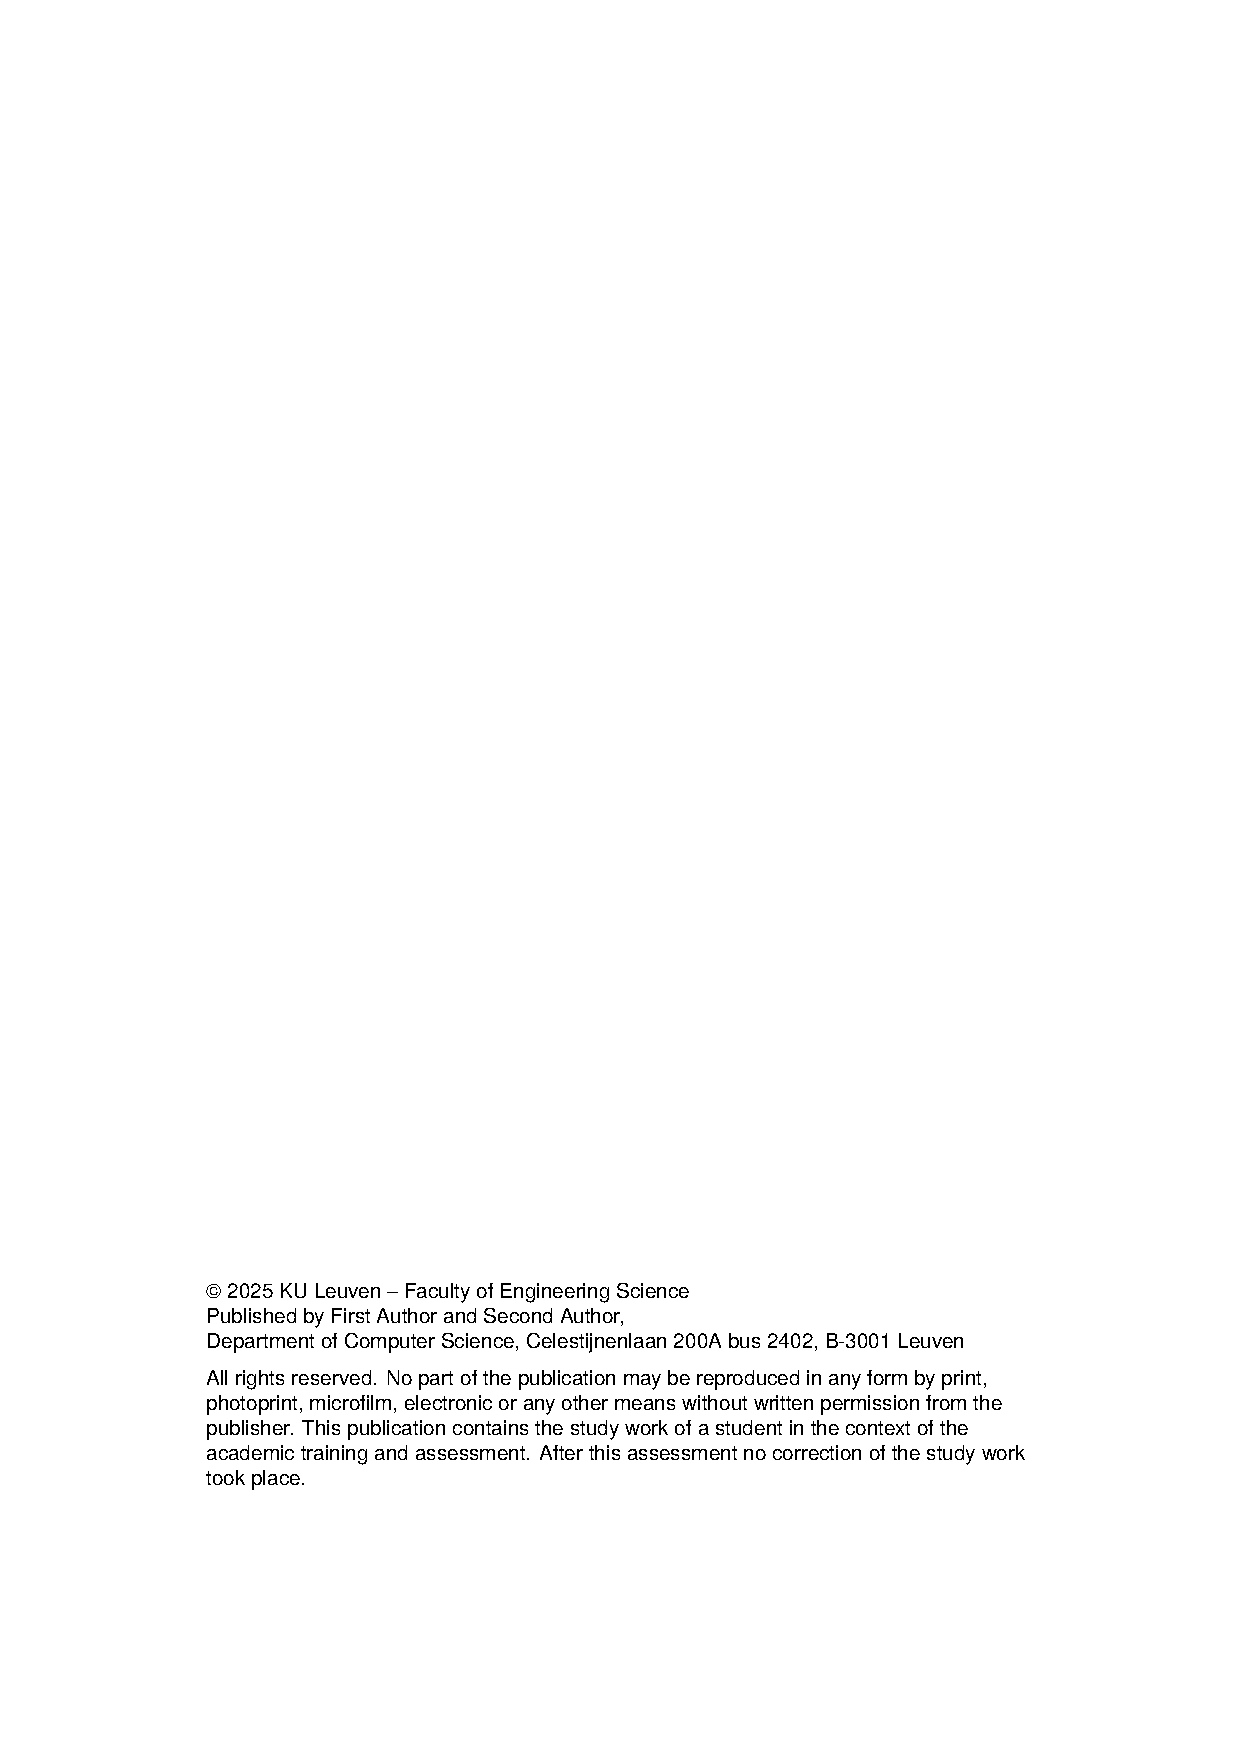
\includegraphics[width=.45\textwidth]{copyright-en}}
  \caption{The official copyright page layout for a Dutch master (left) and an
    English master (right).}
  \label{fig:copyright}
\end{sidewaysfigure}

\section{Front matter}
The front matter contains introductory material such as a preface, an
abstract, and content lists (table of contents, list of tables, list of
figures, list of symbols, etc.).

\paragraph{Preface (\Dutch{\prefacename})} The preface page contains personal
comments from the author(s). The preface can also be used for general
acknowledgements and to express one's thanks. This page is recommended but
not required.

\paragraph{Table of contents (\Dutch{\contentsname})} The table of contents
should be a clear representation of the breakdown of the chapters and the
respective page numbers. Do not show too many levels here since it will make
you loose the reader. So either restrict the table of contents to the
chapter and the section level or add the subsection level in an
unobtrusive way.

\paragraph{Abstract (\Dutch{\abstractname})} The abstract page gives a one
page overview of the work emphasising the results. Try to avoid uncommon
terminology, which will only be defined in the main text later on.

If the master's programme language differs from the main text language, a
second abstract page is needed, which is written in the master's programme
language. This is common practice for Erasmus students, where the main text
language is determined by the host institute. However if the master's programme
guidelines require a multi-page abstract with figures, it's probably better to
put it into an appendix or into an additional chapter in the back matter.

\paragraph{List of figures (\Dutch{\listfigurename})} This list contains for
each figure its sequence number, its caption and its page number. Such a list
is often of limited use in a master's thesis. Therefore it's not required nor
recommended unless the master's programme guidelines require or recommend it.

\paragraph{List of tables (\Dutch{\listtablename})} This list contains
for each table its sequence number, its caption and its page number. The same
remark as for the list of figures is valid here.

\paragraph{Nomenclature (\Dutch{L\ij st van symbolen})} This list holds the
nomenclature of the text. It shows all used symbols and abbreviations and
their meaning. Also conventions such as ``\emph{vectors are printed in
  bold}'' can be put in this list. This list is not required, but it is
recommended if some non-evident symbols or abbreviations are used. It's
useless to have a list of symbols indicating that $\alpha$ means the Greek
letter alpha!

\section{Main matter}
The main matter forms the heart of the thesis text: it contains the real
content. One should be able to read only the main matter to take in the
whole story. The main matter is divided into chapters, which are the
logical entities of the text. The chapters have a logical sequence, which
must be made evident to the reader.

\paragraph{First chapter} In this general introduction the reader must be
informed about the research field of the master's thesis, situating it in a
broader context. The goals of the thesis, as well as previous work, are
described from a technical point of view. The structure of the thesis text
is briefly explained.

\paragraph{Other chapters} Each chapter, except the first and the last one,
starts with an introduction to the contents of the chapter. If readers
would only read the introductions, they should have an overview of the
contents of the master's thesis and the relation between the chapters.

Since chapters form a logical unit, it's expected that conclusions can be
drawn at the end of each chapter about the work described in it. A
concluding section can also help to link a chapter to the next one.

\paragraph{Last chapter} The general conclusion summarises all results,
criticises the methods used, and makes suggestions for further work. It
cannot contain any new elements.

\paragraph{Appendices (\Dutch{B\ij lagen})} The appendices clarify or
complete the text but are not an essential part of the work. Extra
information which is essential for future work is also included in
appendices. Typical examples are: programme code and algorithms, detailed
schematics, equipment specifications, mathematical derivations and an
exhaustive argumentation.

If the master's programme guidelines give a page limit for the text, it
usually only includes the regular chapters, not the appendices. However
appendices cannot be used to bypass this page limit because the evaluation of
the thesis is mainly based on the regular chapters.

\section{Back matter}
The back matter conveys information ancillary to that in the main matter.
Typical examples are a bibliography and a glossary.

\paragraph{Bibliography} The bibliography lists all referenced material. The
format used for the bibliography items is probably determined by the master's
programme guidelines or by the thesis supervisor. References are needed for all
statements that are not proven in the thesis. However references to courses are
superfluous.

\chapter{Typography}
A good first overall impression is always very important. Therefore
typography is a very important part of any masterpiece of text. And isn't
your master's thesis a masterpiece?

Several good books have been written about typography and book design. A
(not so) short overview is found in the Memoir design notes\,\cite{memdesign}.

\section{Basic principles}
The text must be written in a correct language, used in a consistent way.
Spelling mistakes are unacceptable, so at least use a decent spelling
checker. When in doubt, consult a dictionary or an official word list
(known in Dutch as the \Dutch{Groene Boekje}\,\cite{grboek}). A consistent
spelling implies that either British or American spelling is used when
writing an English text.

Consistency is also required for the grammar. Some sources suggest to use a
passive voice such as ``the results are found \ldots''. Other sources
suggest to rather use an active voice such as ``we found this result
\ldots''. Whatever you use, always try to stick to the same kind of
construction.

The master's thesis should be written in a very readable way because it is
meant to communicate the results and scientific experience of the authors
to others.
Since a master's thesis is a scientific work, official metric units (a.k.a.\
SI~units\,\cite{siunits}) must be used.
Identical concepts should be described with identical words or identical
symbols, as well in the body text and equations as in figures and tables.
To help the reader, it may be useful to add a list of symbols and
abbreviations in the front matter.

One sentence should not contain more than one thought and is
therefore short. Ideas that belong together are kept together in one
paragraph. Therefore a paragraph usually contains at least two sentences,
spanning at least two lines.

\section{Fonts}
The body text is typically typeset using a proportional serif typeface. Well
known examples are Times\footnote{Since the typeface Times was developed for
  newspapers with small columns, it is not a good typeface for single column
  texts on A4 paper!} (or Times New Roman), Cambria, Palatino (or Book
Antiqua), Garamond, Utopia, Charter, and Minion. The font used in formulas,
figures, and tables must be the same as the body text font. Symbols in the text
and in formulas must be compatible with the chosen body text font.

A general rule in typography is: \emph{``using fewer typefaces usually means
  better readability''}. But it makes sense to add one or two extra
typefaces for specific types of data to identify them more easily in
running text. To represent the name or contents of a file or a screen, one
typically uses a fixed width font, such as Courier or Consolas. For
non-body text (e.g., titles, headers, footers, captions) a proportional
sans serif font is sometimes used. Well known examples are Helvetica (or
Arial), Calibri, Univers, and Myriad. Just in case you're curious about it,
the fonts used in this document are \rmfontname, \textsf{\sffontname}, and
\texttt{\ttfontname}.
.

A font size of 11\,pt or 10\,pt with a proper leading\,\footnote{Leading is
  the vertical space between two lines of text. The line spacing is the
  font size plus the leading.} must be used for text and symbols. On A4
paper the 11\,pt size is preferred. If you do not know the proper leading
for your font, choose 2.5\,pt for the 11\,pt font and 2\,pt for the 10\,pt
font. Headings can be made more attractive and outstanding by typesetting
them in a larger font size and/or italics or bold.

\section{Layout}
The text is printed on both sides of A4 paper with odd numbered pages on the
recto\,\footnote{The recto page is the right-hand page of a printed book. The
  left-hand page is called the verso page.} side. This implies that the inner
margins (left on recto, right on verso) are smaller than the outer margins, as
shown on \fref{fig:spread}. Contrary to printed books, electronic versions are
often only read from the screen, one page at a time. In the latter case it
makes more sense to have equal left and right margins.

\begin{figure}
  \centering
  \begin{minipage}[b]{0.5\textwidth}
    \drawaspread{0.5\textwidth}{1.5}{1.5}{0.111}{1.5}{2.0}{0}
  \end{minipage}
  \caption{In a spread, showing a recto and a verso page, the combination of
    the two inner margins is perceived as a single margin. Therefore the width
    of an outer margin is comparable to two times the width of an inner
    margin.}
  \label{fig:spread}
\end{figure}

A page contains a single column typeblock and optionally a header and a
footer. The typeblock contains the regular text, the tables and figures,
and the footnotes. To improve the readability of the text, the width of the
typeblock is limited to 14\,cm when using an 11\,pt font and to 13\,cm when
using a 10\,pt font.

The pages should be numbered consecutively, except for the front pages. It
is customary for front matter pages to use lowercase roman numerals and for
other pages to use arabic numerals. In this case the page number is reset
to~1 on the first page of the main matter.

Only chapters in the main matter are numbered: regular chapters with arabic
numerals and appendices with uppercase letters. Chapters in the front and
back matter are unnumbered.
Numbered chapters normally start on a recto page in a printed text.
Inside a chapter, only sections and subsections are numbered, always with
arabic numerals. Too many document levels will confuse the readers instead of
helping them.

One should be able to unambiguously interpret the figures, tables and equations
and they should be numbered. Each reference to equations, figures, and tables
should mention the corresponding number. Each figure should have a caption
below it which briefly indicates what is shown. The main text should refer at
least once to each figure and its content should be discussed in the text. The
author must do the interpretation of the figures, not the reader. The same is
true for tables, but traditionally the table caption is put above the table.

\chapter{Master's programme specific data}
\ReadConfigFile

This section describes some master's programme specific data as it was known on
\PrintConfigFileDate.

\section{List of the masters and their options}
In the academic year \PrintConfigFileAcYr\ these are the masters of the Faculty
of Engineering Science.

\subsection*{Dutch initial master’s programmes}
\ListMastersAndOptions{initial}{dutch}

\subsection*{English initial master’s programmes}
\ListMastersAndOptions{initial}{english}

\subsection*{Advanced master’s programmes}
\ListMastersAndOptions{advanced}{}

\section{Specifying the master's programme option}
Most master's programmes allow you to specify your option (\Dutch{optie}) or
major topic (\Dutch{afstudeerrichting}) of the master's degree, if you want.
But there are some exceptions.
\begin{itemize}
\ListMastersWithOptionType{required}{%
  \item The following master's programmes are known to \emph{oblige} you to
    mention the option or major topic on the title page:}
\ListMastersWithOptionType{forbidden}{%
  \item The following master's programmes are known to \emph{disallow} you to
    mention the option or major topic on the title page:}
\end{itemize}

\bibliographystyle{abbrvurl}
\bibliography{references}

\end{document}

%%% Local Variables: 
%%% mode: LaTeX
%%% TeX-PDF-mode: t
%%% ispell-local-dictionary: "british"
%%% End: 
